\documentclass[a4paper,11pt,twoside]{IT-CNEA}
\usepackage[utf8]{inputenc} % para cambiar el encoding
\usepackage{multicol}

%%%%%%%%%%%%%%%%%%%%%%%%%%%%%%%%%%%%%%%%%%%%%%%%%%%%%%%%%%%%%%%%%%%%%%%%%%%
%               Parametros principales del documento                      %
%%%%%%%%%%%%%%%%%%%%%%%%%%%%%%%%%%%%%%%%%%%%%%%%%%%%%%%%%%%%%%%%%%%%%%%%%%%

% Titulo
\titulo{Propagación de ruido en sistema LTI}
%
% Titulo alternativo para el encabezado
\alttitulo{Elementos de matemáticas aplicada para aplicaciones tecnlógicas}

% Autores
\autores{Augusto Conrado Sardá}{}

% Revisores
\revisores{Jose Relloso}{Agustín Casquero}{}

% Revision de calidad
\calidad{}

% Aprobacion
\aprobacion{}

%Objetivo
\objetivo{}
% Alcance
%\alcance{}

% Numero de informe tecnico
\numeroIT{TP Nº3}
% Metadatos para pdf
\hypersetup{
    pdfauthor={Augusto Conrado Sardá},
    pdftitle={FiltroDeKalmanDeOrientación},
    pdfkeywords={},
    pdfcreator={},
    pdfsubject={}    
    }
    
% Autores de revisiones
%\definechangesauthor[name={Johann Sebastian Mastropiero}, color=blue]{mas}
\usepackage{units}
\usepackage{fancyvrb}
\begin{document}
    % Creacion de la caratula
%    \portada    
    % Creacion del indice
    \tableofcontents       
    % Comienzo del desarrollo del documento
    \printnomenclature[2cm]

\clearpage  
\newpage
\section{Introducción}
En el presente se pretende comprender filtro de Kalman extendido multiplicativo (MEKF por sus siglas en inglés) para la estimación de actitud. Para esto, se cuenta con un diagrama de simulación brindado por la cátedra. 
\\ Este diagrama de simulación se compone de los modelos de los sensores de giróscopo y de star tracker. El primero es necesario para la propagación del filtro mientras que el segundo para la actualización.
\\ A diferencia del trabajo práctico de Allan variance, el modelo de giróscopo se simplifica. Se consideran sólo las componentes de angle random walk (ARW), rate random walk (RRW) y bias instability (BI). A su vez, se agrega una componente de bias constante. Los valores de éstos parámetros variarán en las distintas simulaciones.
\\ Respecto al modelo del star tracker (ST), se considera que posee una desviación estándar de $0.01\,deg$ en todas las simulaciones. 
\\ En varias oportunidades se hará referencia a las matrices $Q$ y $R$. Estas forman parte de la propagación y actualización de los errores de estimación. Los valores con que estas se inicializan forman parte del comportamiento del filtro. 
\section{Simulación 1}
En esta primer simulación se utiliza como modelo para el giróscopo uno de tecnología ring laser gyro (RLG) pero simplificado, sin RRW ni BI. En la tabla Nº\ref{tabla:modeloGyroRLGSimulaciones123} se muestran los valores de los parámetros. 
\par Para inicializar la matriz $Q$ se estableció $ARW=0.001\,deg/\sqrt{h}$ y $RRW=0.01\,deg/\left( h\sqrt{h}\right)$. El primero debería en teoría coincidir con el valor puesto para el modelo del giróscopo (tabla Nº\ref{tabla:modeloGyroRLGSimulaciones123}), pero se lo modificó bajo la consideración de que es difícil conocer cual es ARW que posee el sensor. Entonces, para inicializar la matriz $Q$ se utilizan valores que con algún criterio representen lo mejor posible al sensor (por lo general, este criterio se obtiene de la interpretación de la hoja de datos). Para el valor de RRW, el valor ingresado es bajo el criterio de que sea "suficientemente chico", puesto que no se puede inicializar $Q$ con RRW nulo.
\begin{table}[h!]
\centering
\caption{Modelo del giróscopo para las simulaciones 1, 2 y 3}
\label{tabla:modeloGyroRLGSimulaciones123}
\begin{tabular}{|c|c|c|}
\hline
Parámetro & Unidad& Valor\\ \hline
ARW&$deg/\sqrt{h}$&$0.015$ \\ \hline
RRW&$deg/\left(h\sqrt{h}\right)$&$0$ \\ \hline
BI&$deg/h$&$0$ \\ \hline
Bias constante&$deg/h$&$0.04$ \\ \hline
%&&&&&& \\ \hline
\end{tabular}
\end{table} 
\par En las Figs. Nº\ref{fig:Simulacion1/KalmanQuaterion} y Nº\ref{fig:Simulacion1/KalmanBias} se observan la evolución de los valores de las ganancias Kalman asociadas a la estimación del cuaternión y del bias. El hecho de alcancen valores estacionarios es un comportamiento esperable del filtro de Kalman. De hecho, existen maneras de calcular estos valores estacionarios de las ganancias ignorando los transitorios. 
\\ En la Fig. Nº\ref{fig:Simulacion1/biasEstimado} se observa la evolución de la estimación del bias y como aproximadamente alrededor de $3000\,s$ converge al valor de bias constante establecido como parte del modelo del giróscopo. Esta convergencia no es estacionaria puesto que el esta sujeto a ruido (¡ruido que se pretende modelar con el modelo del giróscopo!). En la parte superior de la Fig. Nº\ref{fig:Simulacion1/biasEstimadoRMSErrores} se ha calculado el RMS del bias estimado a partir de $3000\,s$ y en la parte inferior el error de este respecto al valor de bias constante establecido. Una evaluación rápida de la Fig. Nº\ref{fig:Simulacion1/biasEstimadoRMSErrores} es que a partir de $3000\,s$, el RMS del bias estimado se encuentra alrededor del bias constante dentro del $9\%$ de error. 
\begin{figure}[h!]
\centering
\includegraphics[width=18cm]{/home/pelotari/Documents/MaestriaIB/Materias/ElementosMatematicaGit/TP2Kalman/SimulacionesV2/Simulacion1/KalmanQuaterion.png}
\caption{Simulación 1: Ganancias de Kalman asociadas al cuaternión estimado}
\label{fig:Simulacion1/KalmanQuaterion}
\end{figure}
\begin{figure}[h!]
\centering
\includegraphics[width=18cm]{/home/pelotari/Documents/MaestriaIB/Materias/ElementosMatematicaGit/TP2Kalman/SimulacionesV2/Simulacion1/KalmanBias.png}
\caption{Simulación 1: Ganancias de Kalman asociadas al bias estimado}
\label{fig:Simulacion1/KalmanBias}
\end{figure}
\begin{figure}[h!]
\centering
\includegraphics[width=18cm]{/home/pelotari/Documents/MaestriaIB/Materias/ElementosMatematicaGit/TP2Kalman/SimulacionesV2/Simulacion1/biasEstimado.png}
\caption{Simulación 1: Bias estimado}
\label{fig:Simulacion1/biasEstimado}
\end{figure}
\begin{figure}[h!]
\centering
\includegraphics[width=18cm]{/home/pelotari/Documents/MaestriaIB/Materias/ElementosMatematicaGit/TP2Kalman/SimulacionesV2/Simulacion1/biasEstimadoRMSErrores.png}
\caption{Simulación 1: RMS del bias estimado y error respecto del bias constante}
\label{fig:Simulacion1/biasEstimadoRMSErrores}
\end{figure}
\begin{figure}[h!]
\centering
\includegraphics[width=18cm]{/home/pelotari/Documents/MaestriaIB/Materias/ElementosMatematicaGit/TP2Kalman/SimulacionesV2/Simulacion1/erroresQuaterniones.png}
\caption{Simulación 1: Errores de los cuaterniones medido y estimado respecto al \textit{real}.}
\label{fig:Simulacion1/erroresQuaterniones}
\end{figure}
\section{Simulación 2}
En esta simulación se inicializa la matriz $Q$ con $ARW=0.001*9\,deg/\sqrt{h}$ y RRW no se modifica. 
\par Las Figs. Nº\ref{fig:Simulacion2/KalmanQuaterion} y Nº\ref{fig:Simulacion2/KalmanBias} se muestran las evoluciones de las ganancias de Kalman. En comparación con las Figs. Nº\ref{fig:Simulacion1/KalmanQuaterion} y Nº\ref{fig:Simulacion1/KalmanBias}, los valores estacionarios de esta segunda simulación resultan mayores a los primeros. Puesto que el filtro propaga valiéndose de la medición del giróscopo, al incrementar ARW en la matriz $Q$ se le está ``indicando'' al filtro que se tiene mayor incertidumbre en la medición de este. Por lo tanto el filtro le dará mayor importancia a la actualización que a la propagación y por lo tanto los valores de las ganancias de Kalman aumentarán. 
\\ En cuánto a la estimación del bias del giróscopo, aproximadamente alrededor de $400\,s$ se observa que converge al valor de bias constante. Por lo tanto, el cálculo del RMS del bias estimado se realizó a partir de este tiempo. En comparación con la simulación anterior es claro como aumentó el porcentaje de error en consecuencia de indicarle al filtro que la incerteza en la medición del giróscopo es mayor. 
% Q 
% q
\begin{figure}[h!]
\centering
\includegraphics[width=18cm]{/home/pelotari/Documents/MaestriaIB/Materias/ElementosMatematicaGit/TP2Kalman/SimulacionesV2/Simulacion2/KalmanQuaterion.png}
\caption{Simulación 2:  Ganancias de Kalman asociadas al cuaternión estimado}
\label{fig:Simulacion2/KalmanQuaterion}
\end{figure}
\begin{figure}[h!]
\centering
\includegraphics[width=18cm]{/home/pelotari/Documents/MaestriaIB/Materias/ElementosMatematicaGit/TP2Kalman/SimulacionesV2/Simulacion2/KalmanBias.png}
\caption{Simulación 2:  Ganancias de Kalman asociadas al bias estimado}
\label{fig:Simulacion2/KalmanBias}
\end{figure}
\begin{figure}[h!]
\centering
\includegraphics[width=18cm]{/home/pelotari/Documents/MaestriaIB/Materias/ElementosMatematicaGit/TP2Kalman/SimulacionesV2/Simulacion2/biasEstimado.png}
\caption{Simulación 2:  Bias estimado}
\label{fig:Simulacion2/biasEstimado}
\end{figure}
\begin{figure}[h!]
\centering
\includegraphics[width=18cm]{/home/pelotari/Documents/MaestriaIB/Materias/ElementosMatematicaGit/TP2Kalman/SimulacionesV2/Simulacion2/biasEstimadoRMSErrores.png}
\caption{Simulación 2:  RMS del bias estimado y error respecto del bias constante}
\label{fig:Simulacion2/biasEstimadoRMSErrores}
\end{figure}
\begin{figure}[h!]
\centering
\includegraphics[width=18cm]{/home/pelotari/Documents/MaestriaIB/Materias/ElementosMatematicaGit/TP2Kalman/SimulacionesV2/Simulacion2/erroresQuaterniones.png}
\caption{Simulación 2:  Errores de los cuaterniones medido y estimado respecto al \textit{real}.}
\label{fig:Simulacion2/erroresQuaterniones}
\end{figure}
\section{Simulación 3}
Para finalizar con este primero juego de simulaciones, ahora se disminuyo ARW en la matriz $Q$ a $ARW=0.001/9\,deg/\sqrt{h}$.
\\ En este caso las ganancias de Kalman alcanzan valores inferiores respecto a las Figs. Nº\ref{fig:Simulacion1/KalmanQuaterion} y Nº\ref{fig:Simulacion1/KalmanBias}. La explicación es la opuesta que en la simulación 2. Ahora, al comunicarle al filtro que se tiene menor incerteza en la medición del giróscopo, la propagación es más significativa y por lo tanto las ganancias de Kalman disminuyen. 
\\ Repecto a la estimación del bias, se tiene un tiempo de convergencia considerablemente mayor. Para calcular el RMS de la Fig. Nº\ref{fig:Simulacion3/biasEstimadoRMSErrores} se tomó a partir de $24000\,s$. Sin embargo, aunque el tiempo de convergencia es mayor, el error disminuye significativamente. 
%Q
%q
\begin{figure}[h!]
\centering
\includegraphics[width=18cm]{/home/pelotari/Documents/MaestriaIB/Materias/ElementosMatematicaGit/TP2Kalman/SimulacionesV2/Simulacion3/KalmanQuaterion.png}
\caption{Simulación 3:  Ganancias de Kalman asociadas al cuaternión estimado}
\label{fig:Simulacion3/KalmanQuaterion}
\end{figure}
\begin{figure}[h!]
\centering
\includegraphics[width=18cm]{/home/pelotari/Documents/MaestriaIB/Materias/ElementosMatematicaGit/TP2Kalman/SimulacionesV2/Simulacion3/KalmanBias.png}
\caption{Simulación 3:  Ganancias de Kalman asociadas al bias estimado}
\label{fig:Simulacion3/KalmanBias}
\end{figure}
\begin{figure}[h!]
\centering
\includegraphics[width=18cm]{/home/pelotari/Documents/MaestriaIB/Materias/ElementosMatematicaGit/TP2Kalman/SimulacionesV2/Simulacion3/biasEstimado.png}
\caption{Simulación 3:  Bias estimado}
\label{fig:Simulacion3/biasEstimado}
\end{figure}
\begin{figure}[h!]
\centering
\includegraphics[width=18cm]{/home/pelotari/Documents/MaestriaIB/Materias/ElementosMatematicaGit/TP2Kalman/SimulacionesV2/Simulacion3/biasEstimadoRMSErrores.png}
\caption{Simulación 3:  RMS del bias estimado y error respecto del bias constante}
\label{fig:Simulacion3/biasEstimadoRMSErrores}
\end{figure}
\begin{figure}[h!]
\centering
\includegraphics[width=18cm]{/home/pelotari/Documents/MaestriaIB/Materias/ElementosMatematicaGit/TP2Kalman/SimulacionesV2/Simulacion3/erroresQuaterniones.png}
\caption{Simulación 3:  Errores de los cuaterniones medido y estimado respecto al \textit{real}.}
\label{fig:Simulacion3/erroresQuaterniones}
\end{figure}
\section{Simulación 4}
En esta simulación se cambia el modelo del giróscopo por uno de tecnología MEMS, aunque se continúa con la simplificación que RRW y BI son nulos. En la tabla Nº\ref{tabla:modeloGyroRLGSimulacion4} se muestran los valores de los parámetros. Y respecto al modelo del ST, este no sufre modificaciones. 
\\ En cuanto a las matrices  $R$ y $Q$, la primera tampoco cambia mientras que la segunda si. Se estable $ARW=3\,deg/\sqrt{h}$ y $RRW=10\,deg/\left( h\sqrt{h}\right)$. En primera instancia se había optado por valores de RRW menores, pero se incurría en tiempos de simulación excesivamente largos.
\begin{table}[h!]
\centering
\caption{Modelo del giróscopo para la simulación 4}
\label{tabla:modeloGyroRLGSimulacion4}
\begin{tabular}{|c|c|c|}
\hline
Parámetro & Unidad& Valor\\ \hline
ARW&$deg/\sqrt{h}$&$1.8$ \\ \hline
RRW&$deg/\left(h\sqrt{h}\right)$&$0$ \\ \hline
BI&$deg/h$&$0$ \\ \hline
Bias constante&$deg/h$&$0.25$ \\ \hline
%&&&&&& \\ \hline
\end{tabular}
\end{table}
\par Como indican los parámetros de la tabla Nº\ref{tabla:modeloGyroRLGSimulacion4}, este tipo de giróscopo es de menor calidad que el RLG. A su vez, con la inicialización dada para la matriz $Q$, las ganancias de Kalman para el cuaternión (Fig. Nº\ref{fig:Simulacion4/KalmanQuaterion}) convergen al cabo de un periodo de muestreo del ST. También, los valores estacionarios de las ganancias de Kalman (Figs. Nº\ref{fig:Simulacion4/KalmanQuaterion} y Nº\ref{fig:Simulacion4/KalmanBias}) son del orden de 1000 veces mayor que en el caso de la simulación. Esto concuerda con el comportamiento que al ser un peor giróscopo, la actualización de la medición del ST del filtro cobra mayor importancia que la propagación mediante el modelo. 
\\ La Fig. Nº\ref{fig:Simulacion4/biasEstimadoRMSErrores} muestra claramente como la peor calidad del giróscopo ha degradado la estimación del bias. De los valores establecidos en la matriz $Q$, puede considerarse que ARW esté sobredimensionado, pero también al poner un alto valor de RRW para ``acelerar'' la convergencia se aumenta el error. Como puede observarse, el valor RMS fluctúa dentro del $80\%$ de error, lo que resulta inadmisible. Finalmente, la Fig. Nº\ref{fig:Simulacion4/erroresQuaterniones} se ratifica el mal desempeño ya que practicamente no hay diferencia entre el error del cuaternión estimado y el medido respecto del real. 
\begin{figure}[h!]
\centering
\includegraphics[width=18cm]{/home/pelotari/Documents/MaestriaIB/Materias/ElementosMatematicaGit/TP2Kalman/SimulacionesV2/Simulacion4/KalmanQuaterion.png}
\caption{Simulación 4:  Ganancias de Kalman asociadas al cuaternión estimado}
\label{fig:Simulacion4/KalmanQuaterion}
\end{figure}
\begin{figure}[h!]
\centering
\includegraphics[width=18cm]{/home/pelotari/Documents/MaestriaIB/Materias/ElementosMatematicaGit/TP2Kalman/SimulacionesV2/Simulacion4/KalmanBias.png}
\caption{Simulación 4:  Ganancias de Kalman asociadas al bias estimado}
\label{fig:Simulacion4/KalmanBias}
\end{figure}
\begin{figure}[h!]
\centering
\includegraphics[width=18cm]{/home/pelotari/Documents/MaestriaIB/Materias/ElementosMatematicaGit/TP2Kalman/SimulacionesV2/Simulacion4/biasEstimado.png}
\caption{Simulación 4:  Bias estimado}
\label{fig:Simulacion4/biasEstimado}
\end{figure}
\begin{figure}[h!]
\centering
\includegraphics[width=18cm]{/home/pelotari/Documents/MaestriaIB/Materias/ElementosMatematicaGit/TP2Kalman/SimulacionesV2/Simulacion4/biasEstimadoRMSErrores.png}
\caption{Simulación 4:  RMS del bias estimado y error respecto del bias constante}
\label{fig:Simulacion4/biasEstimadoRMSErrores}
\end{figure}
\begin{figure}[h!]
\centering
\includegraphics[width=18cm]{/home/pelotari/Documents/MaestriaIB/Materias/ElementosMatematicaGit/TP2Kalman/SimulacionesV2/Simulacion4/erroresQuaterniones.png}
\caption{Simulación 4:  Errores de los cuaterniones medido y estimado respecto al \textit{real}.}
\label{fig:Simulacion4/erroresQuaterniones}
\end{figure}
\section{Simulación 5}
En esta simulación se retorna al modelo del giróscopo de las secciones 1, 2 y 3 y también se le agrega RRW. Ver tabla Nº\ref{tabla:modeloGyroRLGSimulacion5}. En la Fig. \ref{fig:Simulacion5/AllanVariance} se muestra la gráfica de Allan variance ($\sigma(T)$ vs. $T$) del ruido generado. 
\par Comparando las Figs. de ésta simulación con la simulación 1, no se aprecian cambios significativos. De hecho, si se observan las Figs. Nº\ref{fig:Simulacion1/biasEstimadoRMSErrores} y Nº\ref{fig:Simulacion5/biasEstimadoRMSErrores}, en esta última el error resulta ínfimamente menor. Una explicación posible es que en esta simulación el modelo del giróscopo se condice con el modelo utilizado para la propagación. Es decir, éste último contempla las componentes de ARW y RRW  de un giróscopo y el ruido que se está generando se compone justamente de estas dos, montadas sobre un bias constante.
%Q
%q
\begin{table}[h!]
\centering
\caption{Modelo del giróscopo para la simulación 5}
\label{tabla:modeloGyroRLGSimulacion5}
\begin{tabular}{|c|c|c|}
\hline
Parámetro & Unidad& Valor\\ \hline
ARW&$deg/\sqrt{h}$&$0.015$ \\ \hline
RRW&$deg/\left(h\sqrt{h}\right)$&$0.01$ \\ \hline
BI&$deg/h$&$0$ \\ \hline
Bias constante&$deg/h$&$0.04$ \\ \hline
%&&&&&& \\ \hline
\end{tabular}
\end{table}
\begin{figure}[h!]
\centering
\includegraphics[width=18cm]{/home/pelotari/Documents/MaestriaIB/Materias/ElementosMatematicaGit/TP2Kalman/SimulacionesV2/Simulacion5/AllanVariance.png}
\caption{Simulación 5:  Allan variance del modelo del giróscopo}
\label{fig:Simulacion5/AllanVariance}
\end{figure}
\begin{figure}[h!]
\centering
\includegraphics[width=18cm]{/home/pelotari/Documents/MaestriaIB/Materias/ElementosMatematicaGit/TP2Kalman/SimulacionesV2/Simulacion5/biasEstimado.png}
\caption{Simulación 5:  Bias estimado}
\label{fig:Simulacion5/biasEstimado}
\end{figure}
\begin{figure}[h!]
\centering
\includegraphics[width=18cm]{/home/pelotari/Documents/MaestriaIB/Materias/ElementosMatematicaGit/TP2Kalman/SimulacionesV2/Simulacion5/biasEstimadoRMSErrores.png}
\caption{Simulación 5:  RMS del bias estimado y error respecto del bias constante}
\label{fig:Simulacion5/biasEstimadoRMSErrores}
\end{figure}
\begin{figure}[h!]
\centering
\includegraphics[width=18cm]{/home/pelotari/Documents/MaestriaIB/Materias/ElementosMatematicaGit/TP2Kalman/SimulacionesV2/Simulacion5/erroresQuaterniones.png}
\caption{Simulación 5:  Errores de los cuaterniones medido y estimado respecto al \textit{real}.}
\label{fig:Simulacion5/erroresQuaterniones}
\end{figure}
\section{Simulación 6}
A diferencia de la simulación anterior, en esta se agrega al modelo el giróscopo la componente de BI. Ver tabla Nº\ref{tabla:modeloGyroRLGSimulacion6}. En la Fig. Nº\ref{fig:Simulacion6/AllanVariance} se muestra la gráfica de Allan variance ($\sigma(T)$ vs. $T$) del ruido generado. 
\begin{table}[h!]
\centering
\caption{Modelo del giróscopo para la simulación 6}
\label{tabla:modeloGyroRLGSimulacion6}
\begin{tabular}{|c|c|c|}
\hline
Parámetro & Unidad& Valor\\ \hline
ARW&$deg/\sqrt{h}$&$0.015$ \\ \hline
RRW&$deg/\left(h\sqrt{h}\right)$&$0.01$ \\ \hline
BI&$deg/h$&$0.009$ \\ \hline
Bias constante&$deg/h$&$0.04$ \\ \hline
%&&&&&& \\ \hline
\end{tabular}
\end{table}
\par El cambio más significativo de esta simulación es la fluctuación de la estimación del bias. Como puede observarse en la Fig. Nº\ref{fig:Simulacion6/biasEstimado}, este no fluctúa alrededor del valor del bias constante establecido como en las simulación anteriores, si no que con mucha más variación. La Fig. Nº\ref{fig:Simulacion6/biasEstimadoRMSErrores} deja en manifiesto esto con el aumento del error del valor RMS de la estimación del bias (a partir de $1000\,s$).
\\ Esta degradación en la estimación del bias se debe a que el modelo del giróscopo utilizado en las ecuaciones de propagación sólo tienen en cuenta las componentes de ARW y RRW. Luego, al agregar componentes de ruido al modelo del giróscopo que el modelo de propagación no tiene en cuenta, el resultado de este último será más deficiente.  
\\ Finalmente, la Fig. Nº\ref{fig:Simulacion6/erroresQuaterniones} muestra que si bien el error del cuaternión se haya filtrado frente al error del cuaternión medido, existe una mayor fluctuación que en simulaciones anteriores. 
%Q
%q
\begin{figure}[h!]
\centering
\includegraphics[width=18cm]{/home/pelotari/Documents/MaestriaIB/Materias/ElementosMatematicaGit/TP2Kalman/SimulacionesV2/Simulacion6/AllanVariance.png}
\caption{Simulación 6:  Allan variance del modelo del giróscopo}
\label{fig:Simulacion6/AllanVariance}
\end{figure}
\begin{figure}[h!]
\centering
\includegraphics[width=18cm]{/home/pelotari/Documents/MaestriaIB/Materias/ElementosMatematicaGit/TP2Kalman/SimulacionesV2/Simulacion6/biasEstimadoRMSErrores.png}
\caption{Simulación 6:  RMS del bias estimado y error respecto del bias constante}
\label{fig:Simulacion6/biasEstimadoRMSErrores}
\end{figure}
\begin{figure}[h!]
\centering
\includegraphics[width=18cm]{/home/pelotari/Documents/MaestriaIB/Materias/ElementosMatematicaGit/TP2Kalman/SimulacionesV2/Simulacion6/erroresQuaterniones.png}
\caption{Simulación 6:  Errores de los cuaterniones medido y estimado respecto al \textit{real}.}
\label{fig:Simulacion6/erroresQuaterniones}
\end{figure}
\section{Simulación 7}
Esta simulación es análoga a las simulación 6, cambiando el modelo del giróscopo por uno de tecnología MEMS. En la tabla Nº\ref{tabla:modeloGyroRLGSimulacion7} se muestran los parámetros utilizados y en la Fig. Nº\ref{fig:Simulacion7/AllanVariance} se muestra el gráfico de Allan variance.
\begin{table}[h!]
\centering
\caption{Modelo del giróscopo para la Simulación 7}
\label{tabla:modeloGyroRLGSimulacion7}
\begin{tabular}{|c|c|c|}
\hline
Parámetro & Unidad& Valor\\ \hline
ARW&$deg/\sqrt{h}$&$1.8$ \\ \hline
RRW&$deg/\left(h\sqrt{h}\right)$&$0.1$ \\ \hline
BI&$deg/h$&$18$ \\ \hline
Bias constante&$deg/h$&$0.25$ \\ \hline
%&&&&&& \\ \hline
\end{tabular}
\end{table}
\par En esta simulación, al trabajar con un peor modelo de giróscopo, la propagación se deteriora de sobremanera. La Fig. Nº\ref{fig:Simulacion7/biasEstimadoRMSErrores} muestra que la estimación del bias se haya en el orden de dos ordenes de magnitud mayor que el bias constante del modelo ($0.25\,deg/h=0.12\,10^{-5}\,rad/s$). Por lo tanto, los errores de la estimación resultan enormes, como muestra la Fig. Nº\ref{fig:Simulacion7/biasEstimadoRMSErrores}. Y en la Fig. Nº\ref{fig:Simulacion7/erroresQuaterniones} se observa como el error del cuaternión estimado resulta prácticamente igual al del medido.
%Q
%q
\begin{figure}[h!]
\centering
\includegraphics[width=18cm]{/home/pelotari/Documents/MaestriaIB/Materias/ElementosMatematicaGit/TP2Kalman/SimulacionesV2/Simulacion7/AllanVariance.png}
\caption{Simulación 7:  Allan variance del modelo del giróscopo}
\label{fig:Simulacion7/AllanVariance}
\end{figure}
\begin{figure}[h!]
\centering
\includegraphics[width=18cm]{/home/pelotari/Documents/MaestriaIB/Materias/ElementosMatematicaGit/TP2Kalman/SimulacionesV2/Simulacion7/biasEstimado.png}
\caption{Simulación 7:  Bias estimado}
\label{fig:Simulacion7/biasEstimado}
\end{figure}
\begin{figure}[h!]
\centering
\includegraphics[width=18cm]{/home/pelotari/Documents/MaestriaIB/Materias/ElementosMatematicaGit/TP2Kalman/SimulacionesV2/Simulacion7/biasEstimadoRMSErrores.png}
\caption{Simulación 7:  RMS del bias estimado y error respecto del bias constante}
\label{fig:Simulacion7/biasEstimadoRMSErrores}
\end{figure}
\begin{figure}[h!]
\centering
\includegraphics[width=18cm]{/home/pelotari/Documents/MaestriaIB/Materias/ElementosMatematicaGit/TP2Kalman/SimulacionesV2/Simulacion7/erroresQuaterniones.png}
\caption{Simulación 7:  Errores de los cuaterniones medido y estimado respecto al \textit{real}.}
\label{fig:Simulacion7/erroresQuaterniones}
\end{figure}
\section{Simulación 8}
El objetivo de esta simulación es observar como evoluciona la estimación del cuaternión si se detiene la actualización del filtro. Esto es sinónimo de que el ST deje de otorgar mediciones, lo que no significa una situación atípica, como por ejemplo cuando la luna lo obstruye. 
\\ Se simula entonces que por un tiempo de $T=10\,min=600\,s$, el filtro no cuenta con la actualización y por lo tanto los parámetros estimados coinciden con los propagados. Dado que la propagación depende del giróscopo, una parámetro que cobra importancia es
\begin{equation}
\gamma =\frac{ARW\sqrt{T}}{\sigma_{ST}}
\end{equation}
El valor de $ARW\sqrt{T}$ da cuenta de cual es error en que se incurre al propagar el cuaternión durante un tiempo $T$ donde no se cuentan con mediciones del ST. Por lo tanto, cuanto menor sea el valor de $\gamma$  mejor será la propagación del filtro. 
\\ En esta simulación se utiliza un modelo del giróscopo contemplando sólo ARW de tecnología RLG, como indica la tabla Nº\ref{tabla:modeloGyroRLGSimulacion8}. 
\begin{table}[h!]
\centering
\caption{Modelo del giróscopo para la simulación 8}
\label{tabla:modeloGyroRLGSimulacion8}
\begin{tabular}{|c|c|c|}
\hline
Parámetro & Unidad& Valor\\ \hline
ARW&$deg/\sqrt{h}$&$0.015$ \\ \hline
RRW&$deg/\left(h\sqrt{h}\right)$&$0$ \\ \hline
BI&$deg/h$&$0$ \\ \hline
Bias constante&$deg/h$&$0$ \\ \hline
%&&&&&& \\ \hline
\end{tabular}
\end{table}
El valor de $\gamma$ es
\begin{equation}
\gamma=\frac{0.015\left[deg/\sqrt{h}\right]\sqrt{10\left[min\right]}}{0.01\left[deg\right]}=\frac{4.36\,10^{-6}\left[rad/\sqrt{s}\right]\sqrt{600\left[s\right]}}{0.01\frac{\pi}{180}\left[rad\right]}=	0.61
\end{equation}
Bajo esta disposición se realizaron $20$ simulaciones con el objetivo de realizar estadística al parar la actualización del ST. En la Fig. Nº\ref{fig:Simulacion8/SuspensionActualizacion} se muestran todas las simulaciones superpuestas. El objetivo de mostrarlas superpuestas es mostrar que en el intervalo temporal donde no se cuenta con la actualización del ST ($600$ a $1200\,s$), la dispersión de la propagación del cuaternión se encuentra dentro las curvas $\pm ARW\sqrt{T}$ (con el $68.3\%$ de probablidad). A partir de los $1200\,s$ se nota claramente como las estimación vuelven a fluctuar alrededor de cero. 
\begin{figure}[h!]
\centering
\includegraphics[width=18cm]{/home/pelotari/Documents/MaestriaIB/Materias/ElementosMatematicaGit/TP2Kalman/SimulacionesV2/Simulacion8/SuspensionActualizacion.png}
\caption{Simulación 8: Estimación del cuaternión con suspensión de la actualización del ST.}
\label{fig:Simulacion8/SuspensionActualizacion}
\end{figure}
\section{Simulación 9}
A diferencia de la simulación anterior, ahora se trata con el modelo de giróscopo de tecnología MEMS, con los parámetros que indica la tabla Nº
\begin{table}[h!]
\centering
\caption{Modelo del giróscopo para la simulación 9}
\label{tabla:modeloGyroRLGSimulacion9}
\begin{tabular}{|c|c|c|}
\hline
Parámetro & Unidad& Valor\\ \hline
ARW&$deg/\sqrt{h}$&$1.8$ \\ \hline
RRW&$deg/\left(h\sqrt{h}\right)$&$0$ \\ \hline
BI&$deg/h$&$0$ \\ \hline
Bias constante&$deg/h$&$0$ \\ \hline
%&&&&&& \\ \hline
\end{tabular}
\end{table}
El valor de $\gamma$ es
\begin{equation}
\gamma=\frac{1.8\left[deg/\sqrt{h}\right]\sqrt{10\left[min\right]}}{0.01\left[deg\right]}=\frac{5.24\,10^{-4}\left[rad/\sqrt{s}\right]\sqrt{600\left[s\right]}}{0.01\frac{\pi}{180}\left[rad\right]}=	73.5>>1
\end{equation}
\begin{figure}[h!]
\centering
\includegraphics[width=18cm]{/home/pelotari/Documents/MaestriaIB/Materias/ElementosMatematicaGit/TP2Kalman/SimulacionesV2/Simulacion9/SuspensionActualizacion.png}
\caption{Simulación 9: Estimación del cuaternión con suspensión de la actualización del ST.}
\label{fig:Simulacion9/SuspensionActualizacion}
\end{figure}
Si bien la Fig. Nº\ref{fig:Simulacion9/SuspensionActualizacion} muestra que la dispersión de la propagación del cuaternión se haya dentro de las curvas de $\pm ARW\sqrt{T}$, el valor de $\gamma$ resulta inadmisible. En este sentido, si se pretende que $\gamma <1$, no se pueden permitir tiempos de actualización superiores a $110\,ms$, lo que significa un requerimiento exigente para un ST.
%Q
%q
\clearpage
\newpage
\section{Conclusiones}
La realización de este filtro de Kalman de orientación fue posible a que la cátedra otorgó el modelo en Simulink ya funcionando. Por lo tanto, fui un usuario de este y sólo modificaba variables para cambiar por ejemplo, el modelo del giróscopo utilizado o las matrices $R$ y $Q$. El mayor cambio introducido fue incorporar algunas componentes adicionales al modelo del giróscopo. De todas maneras, es un cambio prácticamente insignificativo comparado con la complejidad del diagrama de simulación del filtro.
\par En cuanto a los objetivos propuestos por la cátedra a desarrollar, en mayor o menor medida se han logrado. Por un lado se verificó el comportamiento más intuitivo del filtro de Kalman: si se tiene mayor incerteza sobre error del modelo (en este caso, el error que se presume tener en la medición del giróscopo - matriz $Q$), el filtro le dará mayor importancia a la actualización de la medición y por lo tanto las ganancias de Kalman aumentarán. Por el contrario, si se cuenta con un mejor giróscopo, la propagación resultará más relevante que en el caso anterior y por lo tanto las ganancias de Kalman disminuirán. 
\\ Una alternativa que no se ensayó fue aplicar este mismo razonamiento a la incertidumbre sobre las mediciones del ST, aunque el razonamiento es análogo. Si se presume que se tiene una incerteza mayor en la medición del ST, la actualización se degrada y por lo tanto las ganancias de Kalman disminuirán. Lo opuesto ocurrirá si esta incerteza es menor. 
\par La estimación del bias también se encuentra sujeta a la confianza que se tiene sobre la medición del giróscopo; es decir, a la confianza sobre el modelo de propagación. Si se tiene más confianza y entonces se asumen menores valores de ARW y RRW en la matriz $Q$, la estimación del bias fluctuará menos con la contraparte de tomar un mayor tiempo de convergencia. Contrariamente, si se es más conservativo y se optan por valores mayores de ARW Y RRW, la estimación convergerá más rápido pero con mayores fluctuaciones. 
\par Otro punto a destacar es el modelo del giróscopo utilizado por el filtro para propagar. Este sólo tiene en cuenta las componentes de ARW y RRW, montadas cobre un bias constante. Sin embargo, del trabajo práctico sobre Allan variance se sabe que existen otras componentes para incorporar en el modelo (bias instability, quantization noise, drift rate ramp, etc). De hecho, cuando en la simulación 6 se le agregó al modelo del giróscopo la componente de BI, se observó como la estimación del bias se deterioró. 
\par Una simulación realizada que no se mostraron sus resultados fue la de considerar un desalineamiento en el giróscopo. Lo hecho aquí supone que el sistema de referencia de este coincide con el del ST. Como es natural imaginarselo, prácticamente no existe posibilidad que en la práctica esto suceda así. Sin embargo, al introducir un desalineamiento no se observaron resultados distintos en consecuencia a este cambio. Probablemente haya sido un mal interpretación de los resultados y debería reconsiderarse como trabajo futuro.
\par En este sentido de trabajo futuro, el primero y más urgente es comprender las ecuaciones que gobiernan el diagrama de simulación y ser capaz de reproducirlo de manera propia. Si bien se nos cedió material bibliográfico para poder hacer esto, el tiempo disponible para la realización de este trabajo hizo imposible poder estudiarlo de la manera que amerita. En consecuencia, aunque se comprenda el funcionamiento cualitativo del filtro, resta mucho por aprender. 

%Q
%q
\clearpage
\newpage
\bibliographystyle{asmems4}
\bibliography{biblio}
\end{document}
%\begin{figure}[h!]
%\centering
%\includegraphics[width=8cm]{Figuras/.png}
%\caption{}
%\label{fig:}
%\end{figure}
%\begin{figure*}[t!]
%    \centering
%    \begin{subfigure}[t]{0.5\textwidth}
%        \centering
%        \includegraphics[width=8cm]{Figuras/.png}
%        \caption{}
%        \label{fig:}
%    \end{subfigure}%
%    \begin{subfigure}[t]{0.5\textwidth}
%        \centering
%        \includegraphics[width=8cm]{Figuras/.png}
%        \caption{}
%        \label{fig:}
%    \end{subfigure}%
%    ~ 
%    \caption{}
%    \label{}
%\end{figure*}
%\begin{table}[h!]
%\centering
%\caption{}
%\label{tabla:}
%\begin{tabular}{|c|c|c|}
%\hline
%
%%&&&&&& \\ \hline
%\end{tabular}
%\end{table}


%que